\documentclass{beamer}
\usetheme{Boadilla}

\usepackage{statmath}
\usepackage{amsmath}
\usepackage{subcaption}
\usepackage{amsfonts}
\usepackage{graphicx}
\usepackage[demo]{graphicx}
\usepackage{subfig}
\usepackage{caption}
\usepackage{tabularx}


\usepackage{tablefootnote}
\usepackage{amssymb}
\usepackage{float}
\usepackage[colorinlistoftodos]{todonotes}
\usepackage{geometry}
\usepackage{booktabs}
\usepackage{siunitx}
\usepackage{tabularx}
\usepackage{placeins}
\usepackage{booktabs}
\usepackage{xcolor}
\usepackage{colortbl}
\usepackage{multirow}
\usepackage[acronym]{glossaries}
\usepackage{indentfirst}
\usepackage{algorithm}
\usepackage{algorithmic}





\usepackage[
  backend=biber,
  style=alphabetic,
  maxbibnames=10,
  minalphanames=2,
  citestyle=authoryear-comp, 
  sorting=nyt
]{biblatex}
\addbibresource{biblio.bib}
\usepackage[colorlinks=true,linkcolor=blue,citecolor=blue,urlcolor=blue]{hyperref}
\hypersetup{
    colorlinks=true,
    linkcolor=blue,
    citecolor=blue,
    urlcolor=blue
}



\setbeamertemplate{caption}[numbered]
\title{Prédiction des bagages ratés}
\author{JAYLET Olivier}


\begin{document}
\begin{frame}
  \titlepage
\end{frame}

\begin{frame}{Outline}
    \begin{itemize}
        \item Introduction
        \item Etat de l'art
        \item Le tri bagage et périmètre d'étude
        \item Dataset \& Statistiques descriptives
        \item Modèles utilisés
            \begin{itemize}
                \item Modèles de classification
                \item Modèles de calibration de probabilité
            \end{itemize}
        \item Méthodologie
            \begin{itemize}
                \item Data splitting
                \item Cross validation
                \item Overview
            \end{itemize}
        \item Résultats
        \item Shap values
        \item Conclusion
    \end{itemize}
\end{frame}


\begin{frame}{Groupe ADP \& équipe DGEOY} 

\begin{block}{Groupe ADP}
\begin{itemize}
    \item Leader mondial dans la conception, l'exploitation et le développement d'aéroports.
    \item Environ 105 million de passagers à Paris en 2023.
\end{itemize}
\end{block}


\begin{block}{Equipe "Data \& management" (DGEOY)}
    \begin{itemize}
        \item Equipe créée début 2023.
        \item Fait parti de la direction générale des opérations.
        \item Objectif : exploiter la donnée pour réduire le nombre de bagage ratés.
    \end{itemize}
\end{block}
\end{frame}



    
\begin{frame}{Introduction} 

    Definition : Un bagage est considéré comme étant raté lorsqu'il est vu dans les infrastructure (ADP) après le départ de son vol.\break

    
    \begin{itemize}
    \item Approximativement 3\% de bagages ratés\footnote{Un raté coûte en moyenne 300€ à ADP ou aux companies aériennes}.
    \item Notre équipe DGEOY a pour objectif d'aider à la réduction des ratés, grace à l'exploitation des données : 
        \begin{itemize}
            \item Analyses causale des ratés.
            \item Analyses des journées problématiques.
            \item Exploitation des données de maintenance du trieur. \item \textbf{Modèle de prédiction des ratés} afin de : 
                \begin{itemize}
                    \item Retirer des bagages avec une forte probabilité d'être ratés.
                    \item Créer un nouveau process logistique pour les bagages prédis ratés, afin de réussir à les acheminer à temps.
                \end{itemize}
        \end{itemize}

    \end{itemize}
    
\end{frame}

    
\begin{frame}{Introduction} 
    \begin{itemize}
        \item Contenu de mon étude : 
            \begin{itemize}
                \item Modèle de classification binaire (bagage raté ou réussi)
                \item Une prédiction de probabilité calibrée et interprétable (probabilité qu'un bagage soit raté).
            \end{itemize}
        \item Quand faire tourner mes modèles : 
            \begin{itemize}
                \item A l'entrée des infrastructures ADP (trieur bagage).
            \end{itemize}

    \end{itemize}    
\end{frame}


\begin{frame}{Le tri bagage et périmètre d'étude}
    \begin{figure}[h]
        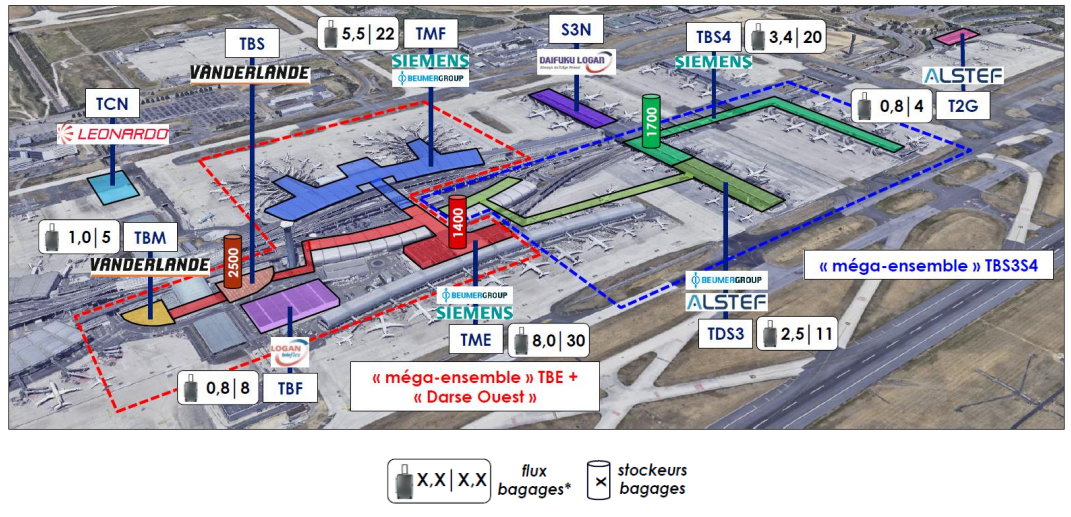
\includegraphics[width=0.7\textwidth]{Plan trieur.png}\\
        \label{fig:Plan trieur}
    \end{figure}
    \begin{figure}[h]
        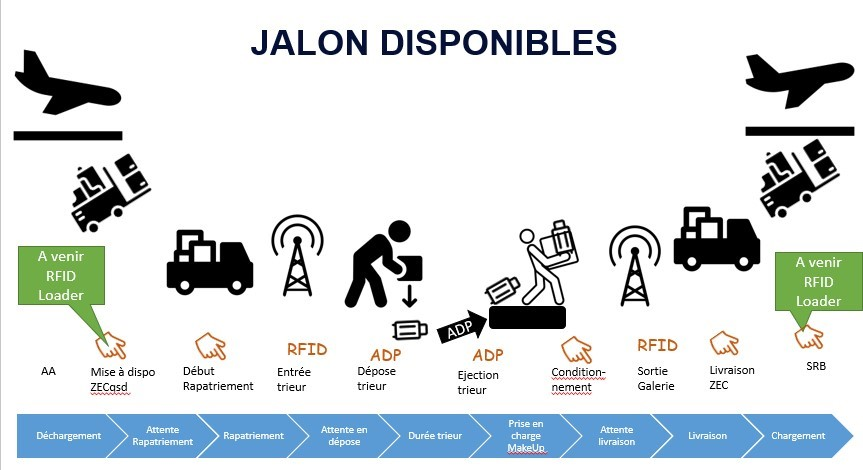
\includegraphics[width=0.7\textwidth]{Jalons tri bagage.jpg}\\
        \label{fig:Les différents jalons du tri bagage}
    \end{figure}
\end{frame}



\begin{frame}{Etat de l'art} 

Plusieurs études de recherche opérationelle trouvées, mais seulement une prédiction des parcours ratés.\hfill \break

\cite{MishandledBgas} a entrainé et testé un Light Gradient Boosting pour prédire les bagages ratés. Le but est d'identifier les bagages "à risque". \hfill \break
\begin{itemize}
    \item Régression logistique comme modèle de référence.
    \item Aucune données provenant du trieur bagage. Seulement des données de la companie aérienne.
    \item Oversampling utilisé pour le problème des données mal-balancées.
    \item Le meilleur modèle a un recall de 0.565, une précision de 0.506 et un F1 score de 0.534.
\end{itemize}
\end{frame}



\begin{frame}{Dataset}

\begin{figure}
        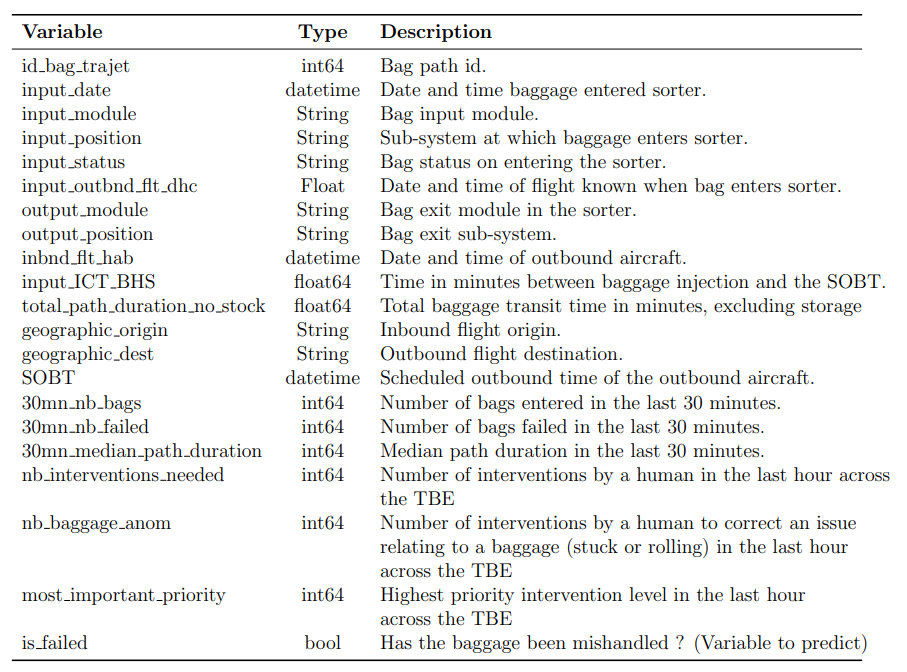
\includegraphics[width=0.7\linewidth]{data table.png}
        \caption{Dictionary of Variables}
\end{figure}

\centering
Date : 1st August 2023 - 31st October 2023

\end{frame}


\begin{frame}{Statistiques descriptives} 
\begin{figure}[ht]
  \centering
  \begin{subfigure}{0.45\textwidth}
    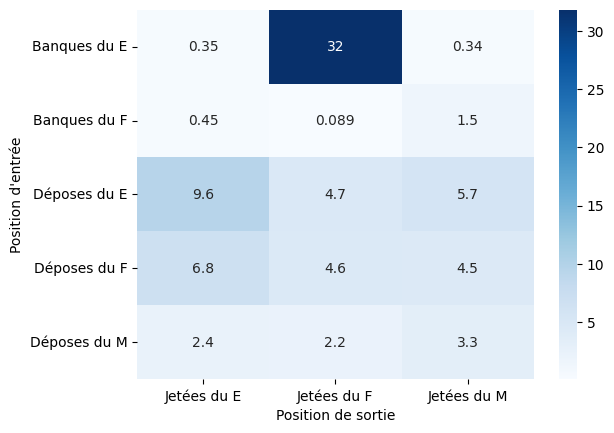
\includegraphics[width=\linewidth]{percentage of failed per positions.png}
    \caption{Pourcentage de bagage ratés en fonction des points d'entrée et de sortie}
    \label{fig:Percentage of mishandled bags according to input and output positions}
  \end{subfigure}
  \hfill
  \begin{subfigure}{0.48\textwidth}
    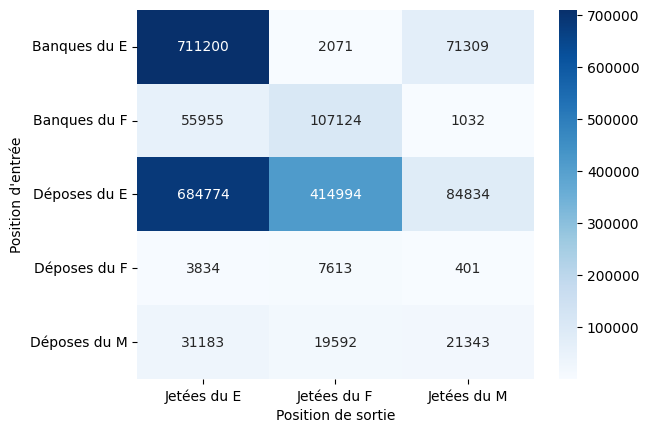
\includegraphics[width=\linewidth]{number of bags per positions.png}
    \caption{Nombre de bagage ratés en fonction des points d'entrée et de sortie}
    \label{fig:Number of bags according to input and output positions}
  \end{subfigure}
  \label{fig:Mishandled bags according to positions}
\end{figure}
\end{frame}



\begin{frame}{Modèles de machine learning entrainés}

\begin{itemize}
    \item Modèles de classification
    \begin{itemize}
        \item Régression logistique (modèle de référence)
        \item Random Forest
        \item XG-Boost
    \end{itemize}
    \item Modèles de calibration de probabilité
    \begin{itemize}
        \item Platt-scaling
        \item Isotonic regression
    \end{itemize}
\end{itemize}
    
\end{frame}


\begin{frame}{Vue globale de la méthodologie}
\begin{figure}[h]
    \centering
    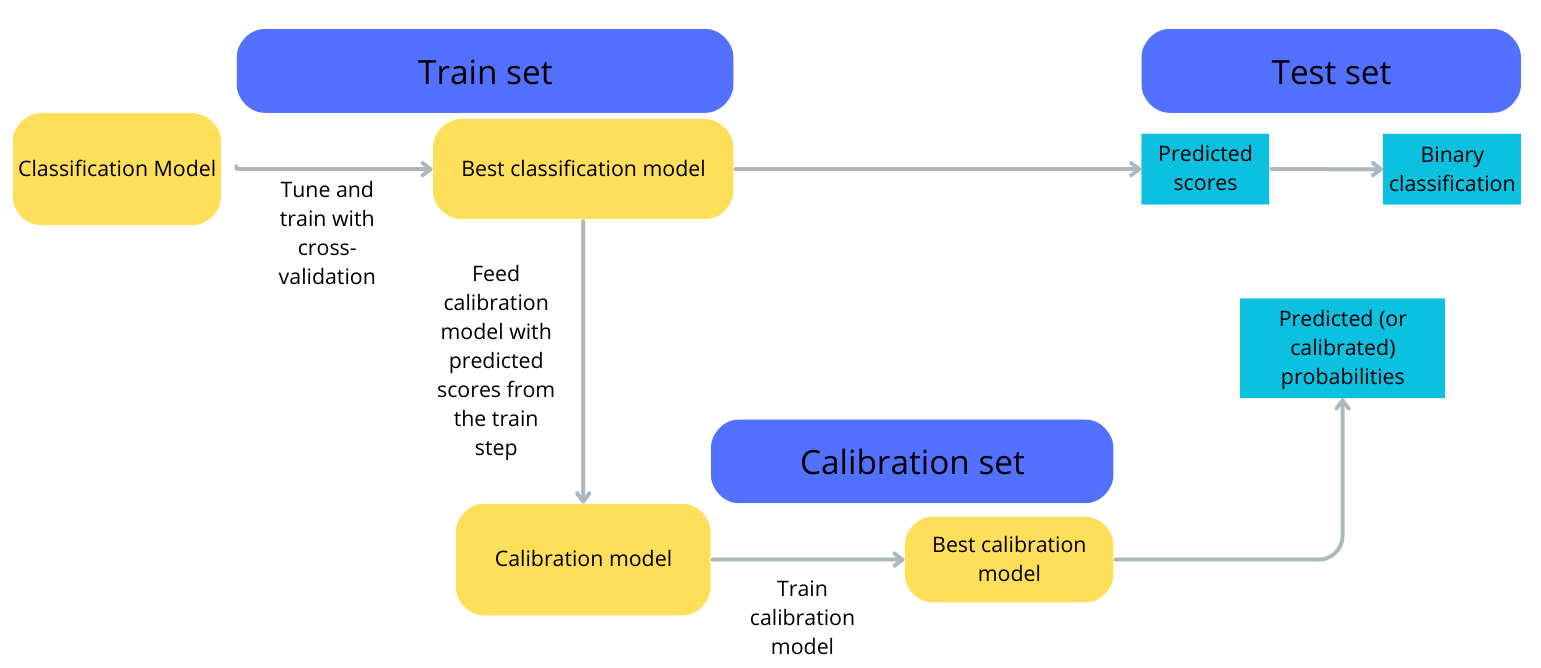
\includegraphics[width=1\textwidth]{Methodology.png}\\
    \caption{Méthodologie d'entrainement, de calibration et de test des modèles}
    \label{fig:Methodogoly}
\end{figure}
\end{frame}



\begin{frame}{Analyse des classifications} 
\begin{figure}
\begin{minipage}[c]{0.4\linewidth}
    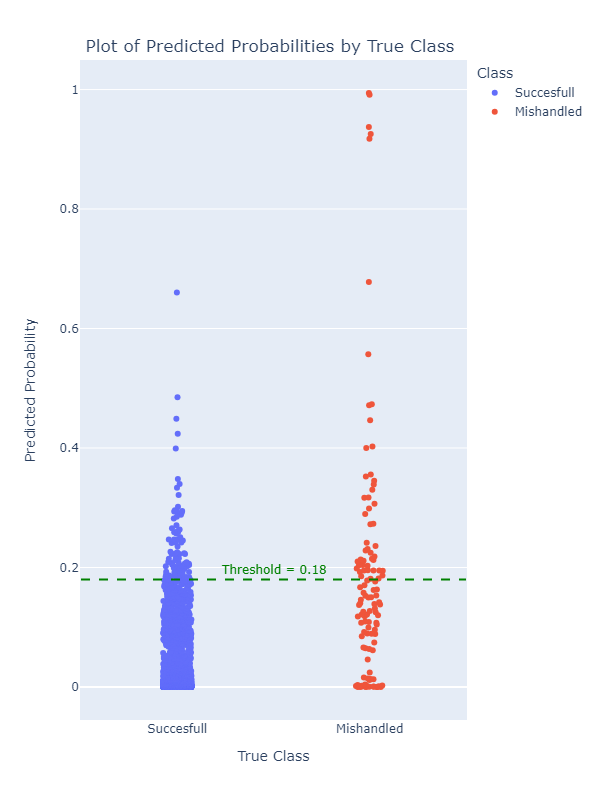
\includegraphics[width=1\textwidth]{Probability_distribution_Model 1.png}\\
    \caption{Distribution des scores prédis - Régression logistique (modèle 1)}
\end{minipage}
\hfill
\begin{minipage}[c]{0.4\linewidth}
    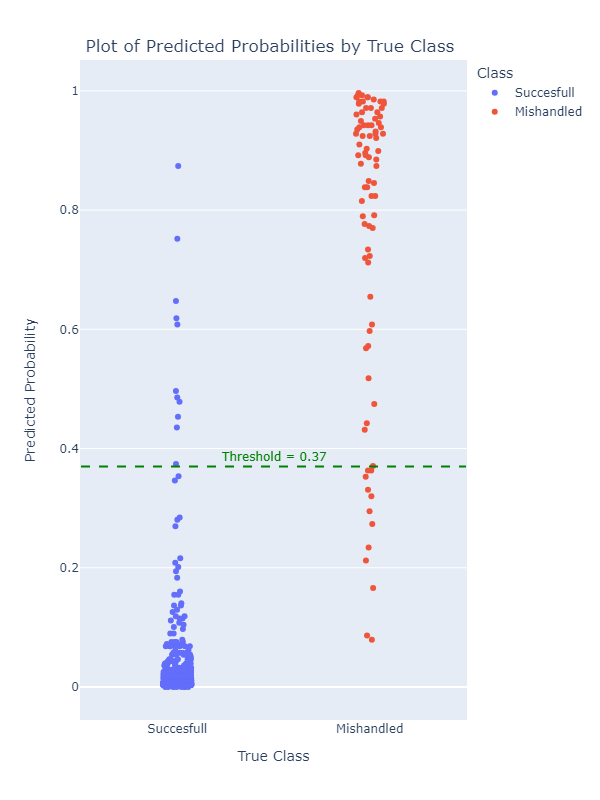
\includegraphics[width=1\textwidth]{Probability_distribution_Model 6.png}\\
    \caption{Distribution des scores prédis - Random Forest (modèle 10)}
\end{minipage}%
\end{figure}
\end{frame}




\begin{frame}{Résultats}

\begin{table}[h]
  \centering
  \caption{Modèles sans les temps de parcours}
  \label{tab:Results}
  \begin{tabular}{|c|c|c|c|}
        \toprule
        \textbf{Model} & \textbf{F1-Score} & \textbf{Recall} & \textbf{Precision}  \\
        \midrule
        Logistic regression & 0,43 & 0.49 & 0.38  \\
        Random Forest & 0.76 & 0.74 & 0.78\\
        XGBoost & 0,74 & 0.73 & 0.75 \\
        \bottomrule
  \end{tabular}
\end{table}


\begin{table}[h]
  \centering
  \caption{Modèles avec les temps de parcours}
  \label{tab:Results}
  \begin{tabular}{|c|c|c|c|}
        \toprule
        \textbf{Model} & \textbf{F1-Score} & \textbf{Recall} & \textbf{Precision}  \\
        \midrule
        Random Forest & 0,88 & 0.85 & 0.9  \\
        XGBoost & 0,89 & 0.87 & 0.9  \\
        \bottomrule
  \end{tabular}
\end{table}
\end{frame}

\begin{frame}{Shapley values}
\begin{figure}[h!]
    \centering
    \begin{subfigure}[b]{0.45\textwidth}
        \centering
        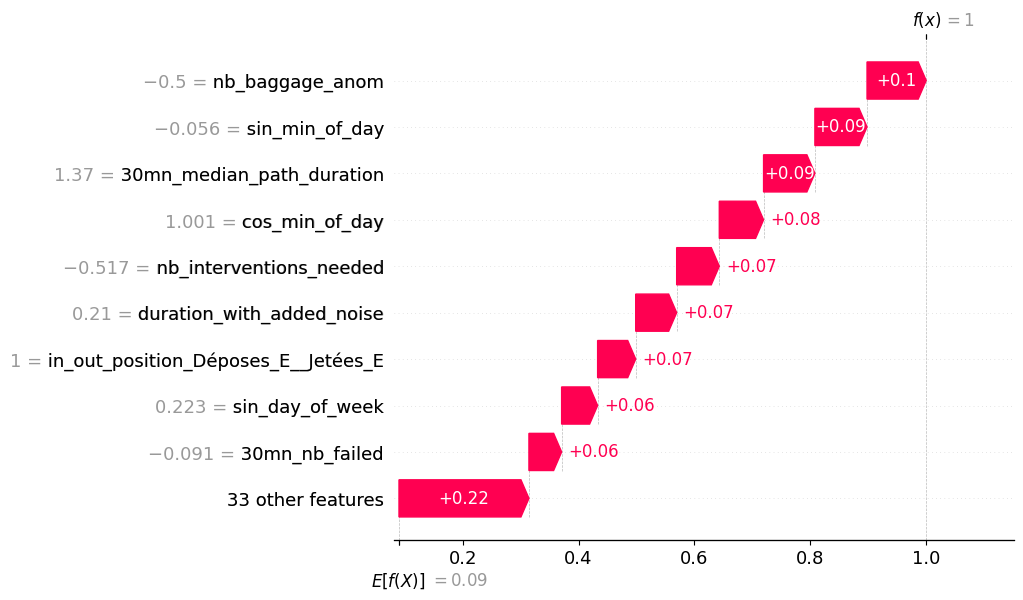
\includegraphics[width=\textwidth]{shap values 1.png}
    \end{subfigure}
    \hfill
    \begin{subfigure}[b]{0.45\textwidth}
        \centering
        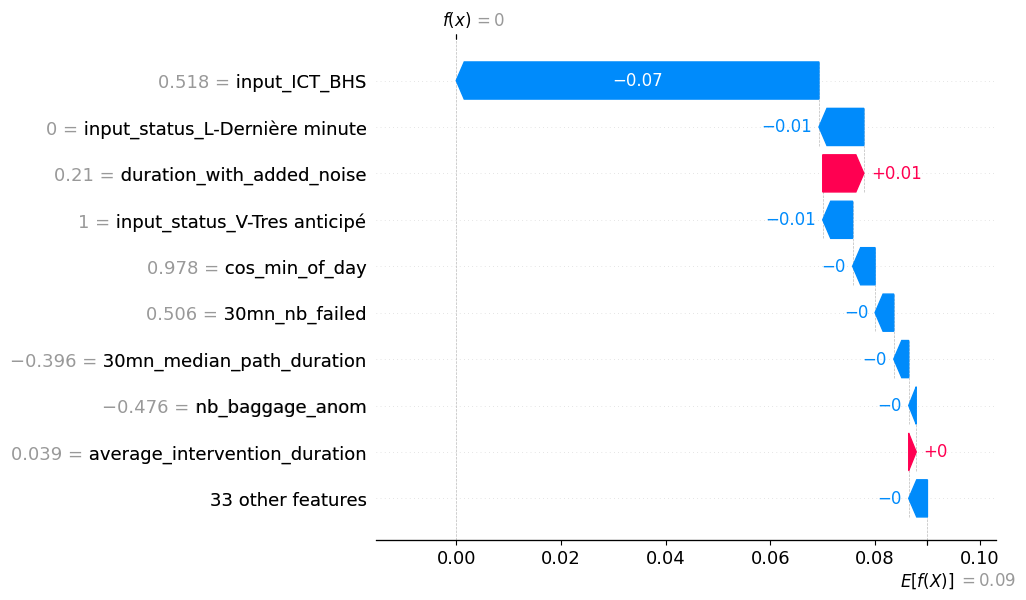
\includegraphics[width=\textwidth]{shap values 2.png}
    \end{subfigure}
    \break
    \begin{subfigure}[b]{0.45\textwidth}
        \centering
        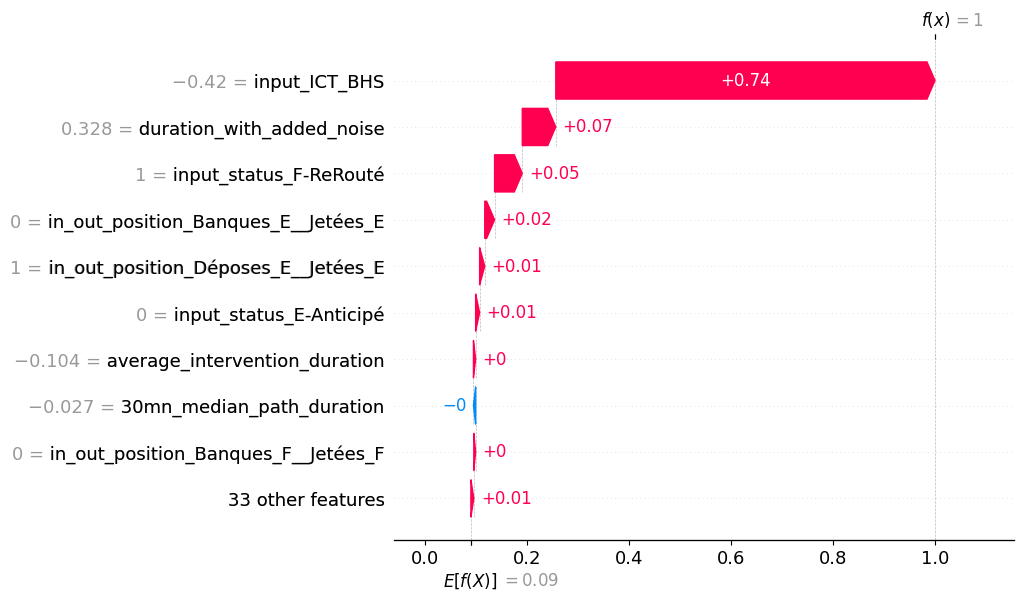
\includegraphics[width=\textwidth]{shap values 3.png}
    \end{subfigure}
    \caption{Shap values pour trois bagages ratés}
\end{figure}
    
\end{frame}




\begin{frame}{Conclusion} 
    \begin{itemize}
        \item Resultats :
            \begin{itemize}
                \item le XGBoost et le Random Forest sont efficaces pour prédire les bagages ratés.
                \item Meilleurs scores que \cite{MishandledBgas}
                \item Mes modèles fournissent une classification accompagnées de probabilités.
                \item Les temps de parcours ont un impact important sur les prédictions.
            \end{itemize}
    \end{itemize}
\end{frame}



\begin{frame}{Conclusion} 
    \begin{itemize}
        \item Limitations :
            \begin{itemize}
                \item Modèles entrainés et testés sur trois mois seulement.
                \item Les temps de parcours ont été générés. Les vraies prédictions n'ont pas été utilisées.
            \end{itemize}
        \item Suggestions d'approfondissement :
            \begin{itemize}
                \item Entrainer les modèles pour une année entière.
                \itemTester les modèles pour des journées avec des forts taux de ratés.
                \item Utiliser les shap values pour des analyses post-ops.
                \item Chercher la meilleure manière d'imbriquer le modèle de temps de parcours au modèle de prédiction de ratés.
            \end{itemize}
    \end{itemize}
\end{frame}




\begin{frame}
  \begin{center}
    \Huge \textit{Merci pour votre attention !}
  \end{center}
\end{frame}


\begin{frame}{Résultat de la calibration de probabilité}
\begin{figure}[h]
    \centering
    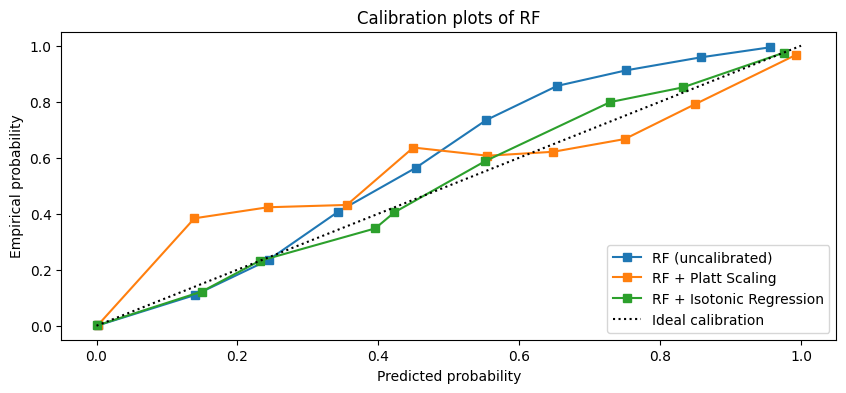
\includegraphics[width=0.8\textwidth]{Calibration_plot_RF.png}\\
    \caption{Calibration pour le random forest}
    \label{fig:Probability calibration for rf}
\end{figure}
\end{frame}


\begin{frame}{Le tri bagage dans le trieur}
    \begin{figure}[h]
    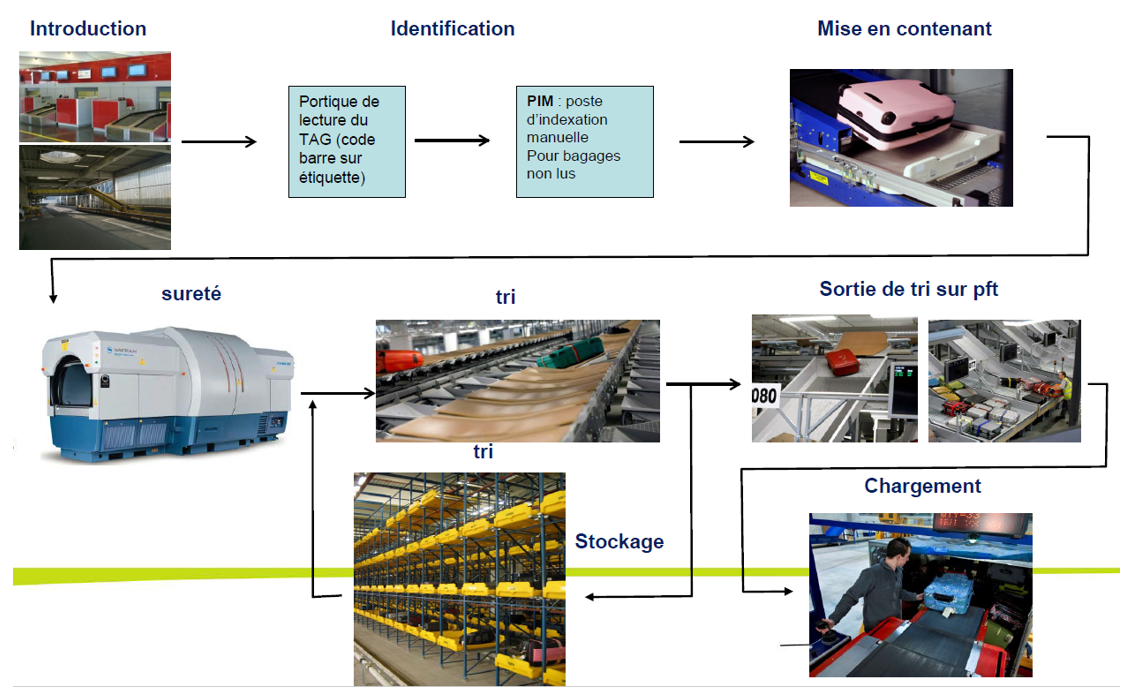
\includegraphics[width=0.9\textwidth]{tri baggage.png}\\
        \label{fig:tri bagage}
    \end{figure}
\end{frame}


\begin{frame}{Confusion matrix}
    \begin{figure}
    \begin{minipage}[c]{0.45\linewidth}
    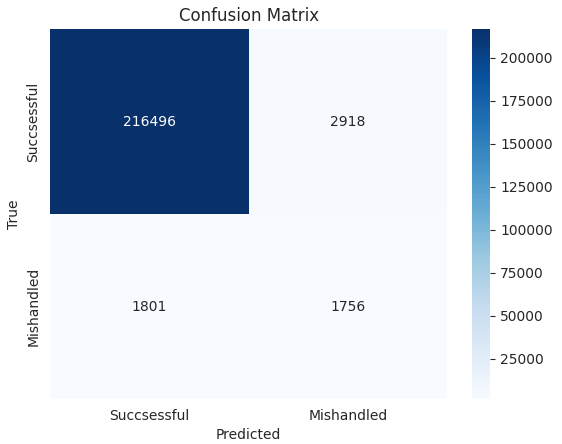
\includegraphics[width=1\textwidth]{Confusion_matrix_Model 1.png}\\
    \caption{Matrice de confusion - LR}
\end{minipage}
\hfill
\begin{minipage}[c]{0.45\linewidth}
    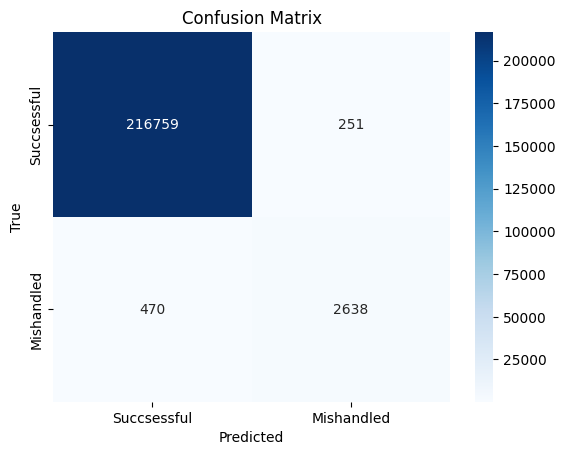
\includegraphics[width=1\textwidth]{Confusion_matrix_Model 6.png}\\
    \caption{Matrice de confusion - RF}
\end{minipage}
\end{figure}
\end{frame}






\begin{frame}{Calibration de probabilité}

Pourquoi calibrer les probabilités ?
\begin{itemize}
    \item Les modèles de ML classifient les données en fonction d'un score prédit (entre 0 et 1).
    \item Ce score ne peut pas toujours être interprété comme une probabilité.
    \item La calibration de probabilité permet de transformer un score en une probabilité.
    \begin{itemize}
        \item Le Platt scaling est une régression logistique sur les scores et la régression isotonique une méthode d'estimation non-paramétrique. 
        \item Les deux prennent les scores prédis comme input et le status raté ou réussi comme variable cible.
    \end{itemize}
\end{itemize}

    
\end{frame}




\begin{frame}{Statistiques descriptives}
\begin{figure}[h]
    \centering
    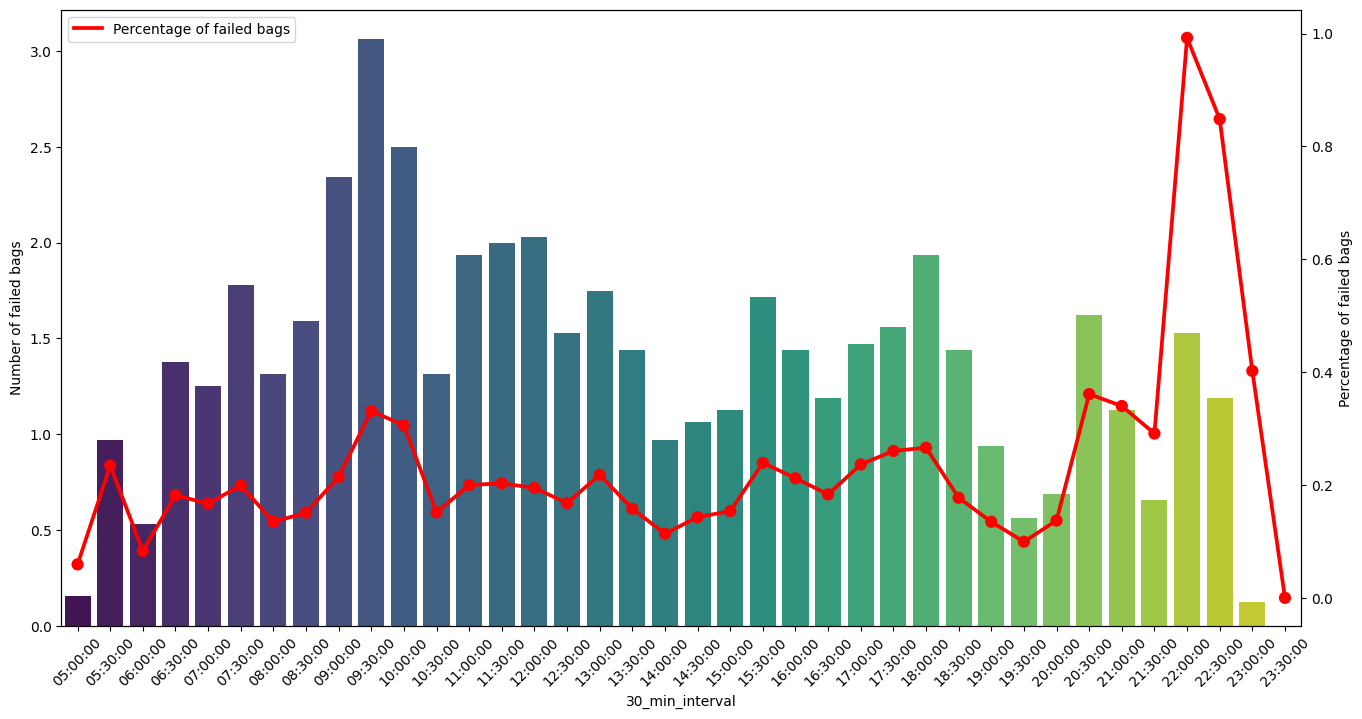
\includegraphics[width=0.9\textwidth]{Number and percentage of failed bags within a day.png}\\
    \caption{Moyenne du nombre de bagage ratés toutes les 30 minutes de la journée}
    \label{fig:Average number and percentage of mishandled bags each 30 minutes of the day}
\end{figure}

\end{frame}


\begin{frame}{Statistiques descriptives}
    \begin{figure}[ht]
      \centering
      \begin{subfigure}{0.48\textwidth}
        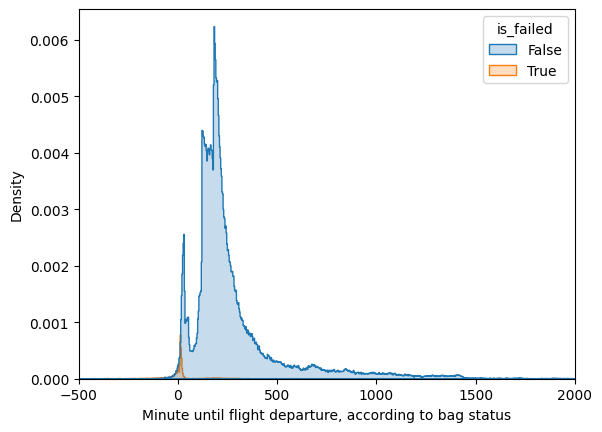
\includegraphics[width=\linewidth]{Minute until flight departure_2.png}
      \end{subfigure}
      \hfill
      \begin{subfigure}{0.48\textwidth}
        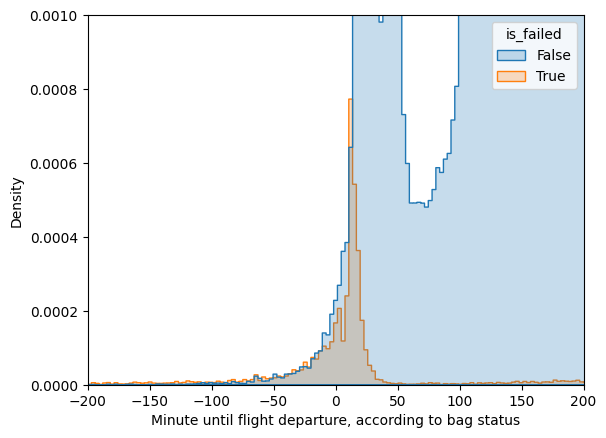
\includegraphics[width=\linewidth]{Minute until flight departure_3.png}
      \end{subfigure}
      \caption{Temps restant en minutes avant le départ prévu du vol\footnote{Au moment où le bagage est injecté dans le trieur, combien de temps reste-t-il avant le départ \textit{planifié} de son vol}}
      \label{fig:Minute until flight departure distribution according to bag status}
    \end{figure}

\end{frame}



\begin{frame}{Methodologie}
\begin{figure}[h]
    \centering
    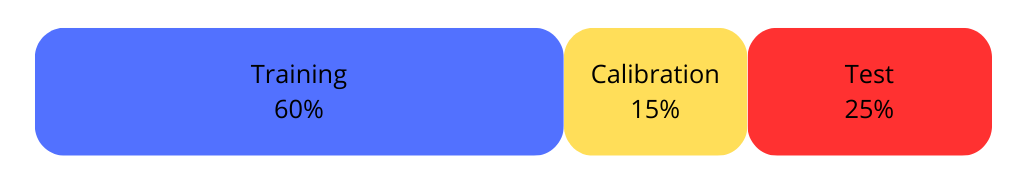
\includegraphics[width=0.7\textwidth]{Data splitting.png}\\
    \caption{Data split}
    \label{fig:Data split}
\end{figure}
\begin{figure}[h]
    \centering
    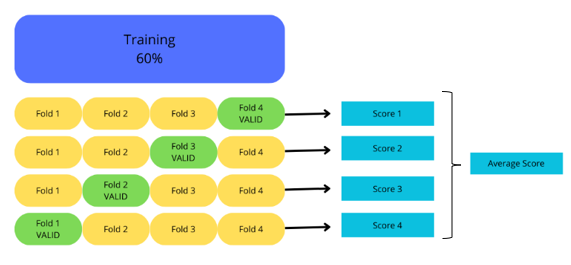
\includegraphics[width=0.65\textwidth]{KFold data.png}\\
    \caption{KFold cross-validation stratifiée}
    \label{fig:KFold cross-validation}
\end{figure}
\end{frame}



\begin{frame}{Path duration impact}
    \begin{figure}[h]
        \centering
        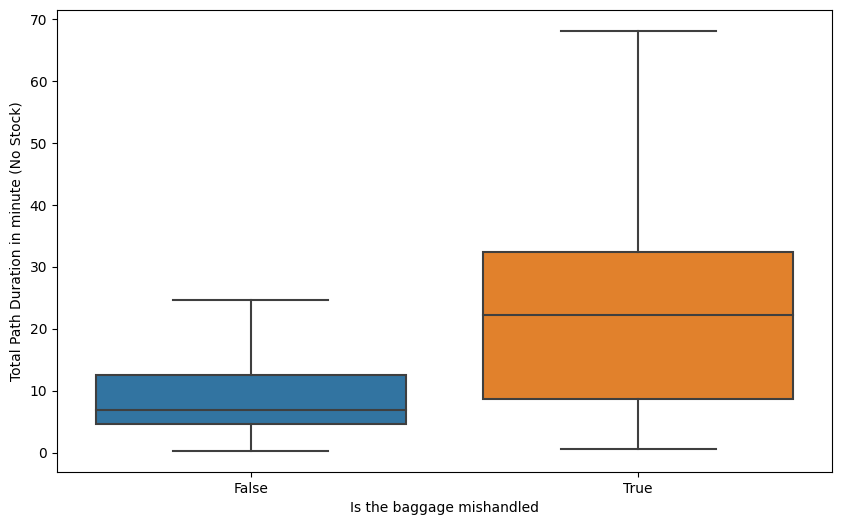
\includegraphics[width=0.6\textwidth]{Boxplot path duration per failed status.png}\\
        \caption{Distribution of paths duration for successful and mishandled bags (without outliers)}
        \label{fig:Distribution of paths duration for non-failed and failed bags}
    \end{figure}
\end{frame}


\begin{frame}{Noise generation on path duration}

\begin{itemize}
    \item Path duration is known once the path exits the BHS.
    \item But path duration can be predicted beforehand (see Miracle's study).
    \item In the future : we could use predicted path duration as a proxy. 
    \item In my study : I generate noise according to path duration prediction residuals, and add them to the actual path duration.
\end{itemize}


\end{frame}





\begin{frame}{Noise generation on path duration} 
\begin{figure}[ht]
  \centering
    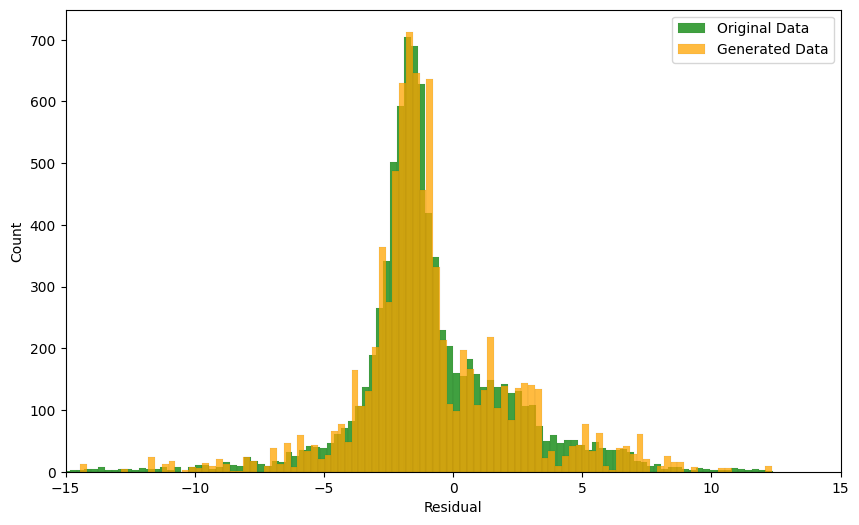
\includegraphics[width=\linewidth]{Q1_Q3 distribution actual Vs. generated.png}
    \caption{Distribution of actual Vs. generated residuals (Q1 $<$ TMP $<$ Q3)}
    \label{fig:Q1_Q3 distribution actual Vs. generated}
\end{figure}
\end{frame}


\begin{frame}{Noise generation on path duration}

\begin{figure}[h]
    \centering
    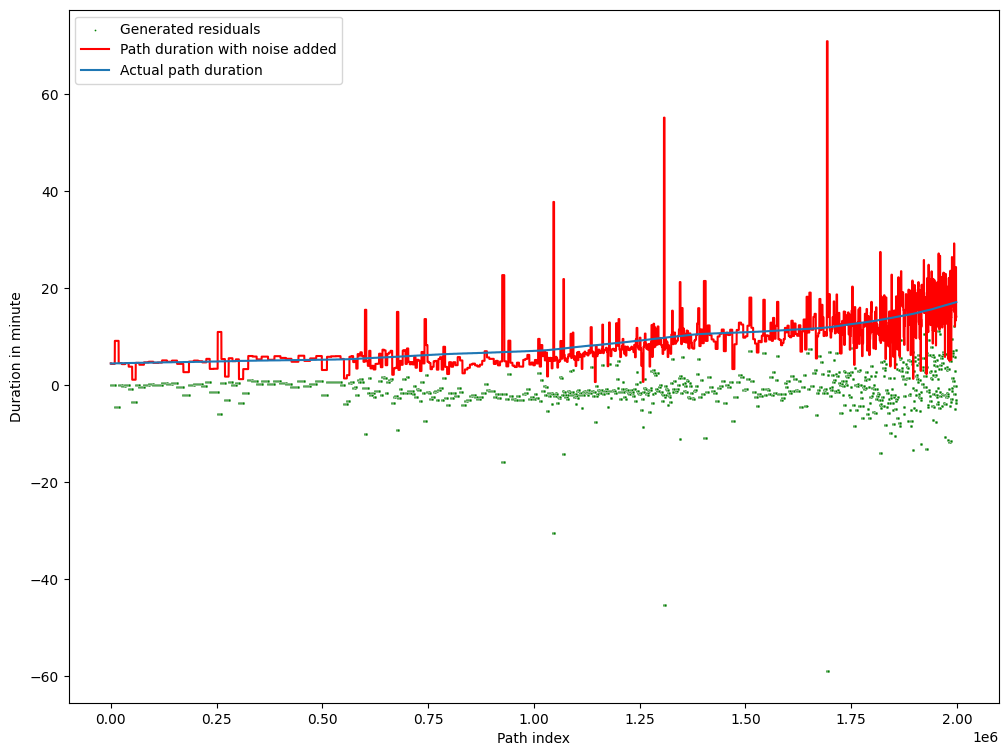
\includegraphics[width=0.8\textwidth]{Q1_Q3 path duration noised.png}\\
    \caption{Comparison of actual path duration with path duration with noise added (Q1 $<$ Path duration $<$ Q3)}
    \label{fig:Q1_Q3 path duration noised.png}
\end{figure}
    
\end{frame}


\begin{frame}{Shap values}
    \begin{figure}[h]
        \centering
        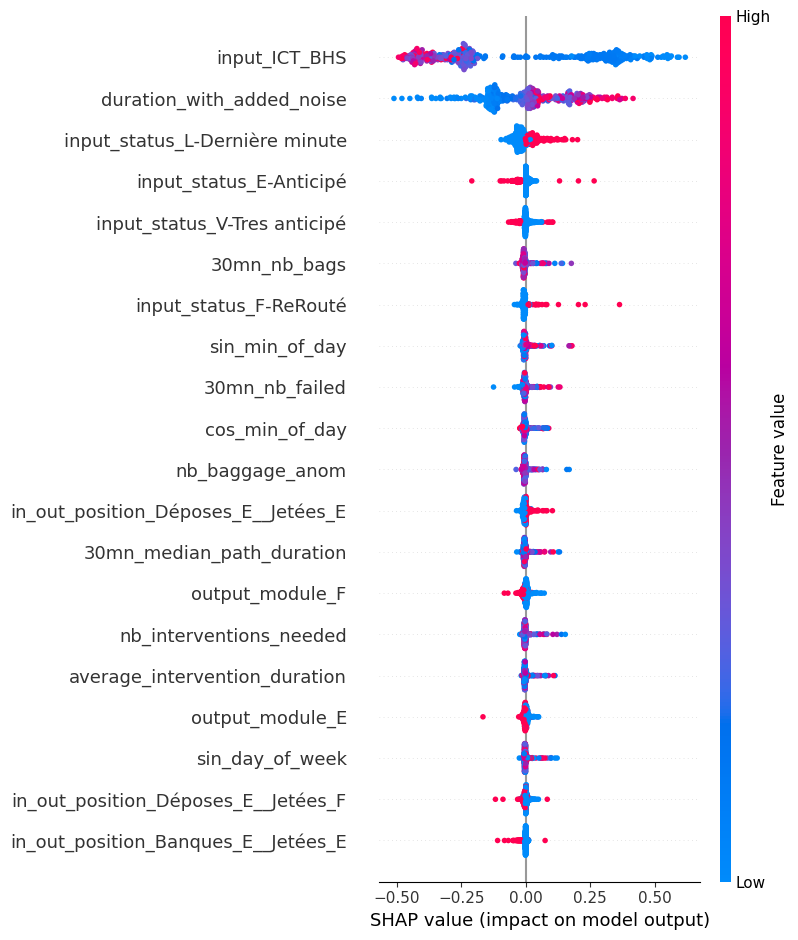
\includegraphics[width=0.5\textwidth]{shap values.png}\\
        \caption{Shap values du modèle 10 (RF + Regression isotonique)}
        \label{fig:Shap values}
    \end{figure}
\end{frame}



\end{document}

